%\documentclass[aps,prl,twocolumn,showpacs,superscriptaddress,groupedaddress]{revtex4-1}  % for review and submission
%\documentclass[aps,preprint,showpacs,superscriptaddress,groupedaddress]{revtex4-1}  % for double-spaced preprint

%Phys Rev B
%Letter or rapid communication - 3500 words
%\documentclass[prb,groupedaddress,reprint]{revtex4-1}
%APL
\documentclass[aps,prl,reprint]{revtex4-1}
%\documentclass[aip,jap,reprint]{revtex4-1}
\usepackage[english]{babel}
\usepackage{graphicx}% Include figure files
\usepackage[pdftex,unicode,colorlinks, citecolor=blue,%
filecolor=black, linkcolor=blue, urlcolor=black]{hyperref}
\usepackage[figure,table]{hypcap} %links should lead to the begining
                                %of figure or table...

\begin{document} %Max size in pdf for APL - 4 print pages

\title{More effective than a ``super'' absorption in spherical nanoparticles}


\author{Konstantin Ladutenko} \email[e-mail: ]{fisik2000@mail.ru}
\affiliation{ITMO University, 49 Kronverskii Ave., St.~Petersburg
  197101, Russian Federation\\}

\affiliation{Ioffe Physical-Technical Institute of the Russian
  Academy of Sciences,
  26 Polytekhnicheskaya Str., St.~Petersburg 194021, Russian
  Federation}

\author{Ovidio Pe\~{n}a-Rodr\'{i}guez} \affiliation{Instituto de
  Fusi\'{o}n Nuclear, Universidad Polit\'{e}cnica de Madrid,\\
  Jos\'{e} Guti\'{e}rrez Abascal 2, E-28006 Madrid, Spain}


% \author{Irina Melchakova}
% \author{Alexander Shalin}
% \affiliation{ITMO University, 49 Kronverskii Ave., St.~Petersburg
%   197101, Russian Federation\\}
%TODO не хватает адреса
% \affiliation{Kotel’nikov Institute of Radio Engineering and
%   Electronics of RAS (Ulyanovsk branch),\\48 Goncharov Str., Ulyanovsk
%   432011, Russian Federation}
% \affiliation{Ulyanovsk State University, 42 L. Tolstoy Str., Ulyanovsk 432017, Russian Federation}
% \author{Ilya Yagupov}
% \author{Pavel Belov}
% \affiliation{ITMO University, 49 Kronverskii Ave., St.~Petersburg
%   197101, Russian Federation\\}
\author{Ali Mirzaei} 
\author{Andrey Miroshnichenko}
\author{Ilya Shadrivov}
\affiliation{Nonlinear Physics Centre, Research School of Physics and Engineering,
The Australian National University, 59 Mills Rd, Acton, ACT, 2601, Australia}

\date{\today}
% APL 250 words! Moreover, some designs have spectral Phys Rev B less
% then 500 words, about 5% ot total paper length
% emacs M-x count-words

\begin{abstract}

  There was some recent fuzz about ``superscattering'' effect, which is
  about to design a structure such a way, that several multiple
  (electric and/or magnetic) resonances are overlapped.  This breaks
  the theoretical limit we can achieve using a single resonance,
  that`s why it is called ``super''. Our initial idea was to show the
  same effect in absorption, and R=63 with R=81nm are such
  `superabsopting` designs. However, in 3D case (in contrast to 2D
  investigated with Ali) it turned out that sometimes it is preferable
  to use a smaller particle with single resonance to achieve the best
  efficiency. This way, in 3D case using real materials for a
  multilayer spherical particle ``superabsorbing'' design do not
  always leads to best absorption efficiency. Moreover, same effect
  exists for scattering from SiAgSi optimized structure. At WL=500 nm
  ``super'' scattering mode with two resonances gives the best
  efficiency, however, at WL=400 nm a single resonance small particle
  has a better scattering efficiency compared to larger particles with
  ``super'' design.
\end{abstract}

\pacs% insert suggested PACS numbers in braces on next line
{41.20.Jb 42.25.Fx 02.60.Pn 02.70.-c}
%41.20.Jb	Electromagnetic wave propagation
%42.25.Fx	Diffraction and scattering
%02.60.Pn	Numerical optimization
%02.70.-c	Computational techniques; simulations 

\maketitle %\maketitle must follow title, authors, abstract and \pacs
% \section{Introduction}
% Interest in metamaterials, artificial media with exotic
% electromagnetic properties, has increased considerably during the
% past decade.~\cite{Smith-2004, Schurig-2006, Shalaev-2007,
%   Kivshar-2012, ufn-ru-2015} One of the best known applications of
% metamaterials is cloaking.  Usually, invisibility cloaks are
% designed using transformation optics (TO) concept~\cite{pendry_TO,
%   Leonhardt-2006} and involve metamaterials with anisotropic,
% magnetic, and extreme material parameters.

% There are some recent efforts to achieve cloaking using isotropic
% dielectric materials readily available in
% nature~\cite{Sigmund-AllDiel-2011, smith-3dprinterCloak-2013,
%   Fujii_topolOpti_theory_2013, Lan-unidir-2D-cloak-ALP-2013,
%   semouchkina2}, mostly resulting in designs of unidirectional
% cylinder cloaking.  Another approach~\cite{Takezawa-AIP-2014} is to
% combine isotropic dielectric materials to obtain anisotropic properties
% after homogenization of a multilayer cylinder cloak.  Designs with
% sphere symmetry using multilayer dielectric
% coating~\cite{semouchkina_sphere_multilayer, Ladutenko-2014} have been
% obtained using stochastic optimization methods.

\begin{figure}
  \center{
    % Use pdfcrop to remove white margins
    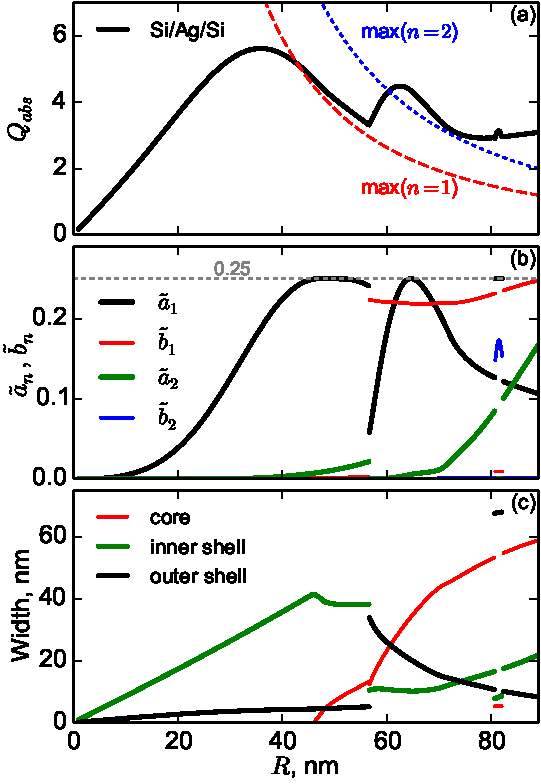
\includegraphics[width=0.47\textwidth]{fig/2015-04-01-Qabs-SiAgSi-overview}%
    \caption{ Optimized designs overview at working wavelength
      $\lambda = 500$~nm. (a) Expansion
      coefficients (b) Absorption efficiency with best value at total
      R=36~nm and Ag/Si design (zero sized core) and ``super'' designs
      at R=63~nm and R=81~nm. (c) Used layers width
      %\label{fig:model-view}
    }%
  }
\end{figure}

\begin{figure}
  \center{
    % Use pdfcrop to remove white margins
    \includegraphics[width=0.47\textwidth]{fig/2015-04-01-SiAgSi-ab-spectra2.pdf}%
    \caption{
      Expansion coefficients spectra of (a) efficient and (b)
      ``super'' design.
      %\label{fig:model-view}
    }%
  }
\end{figure}

\begin{figure}
  \center{
    % Use pdfcrop to remove white margins
    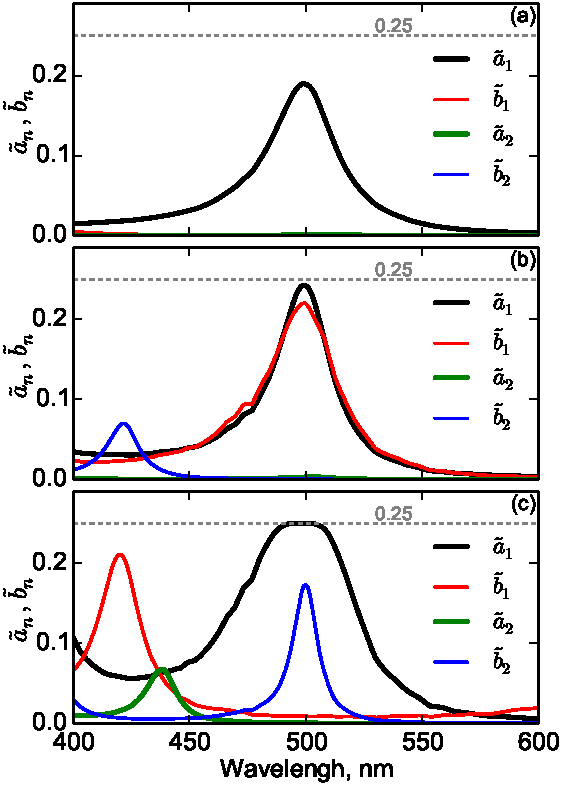
\includegraphics[width=0.47\textwidth]{fig/2015-04-01-SiAgSi-ab-spectra3.pdf}%
    \caption{
      (Or we can use)
      Expansion coefficients spectra of (a) efficient and (b-c)
      ``super'' design.      
      %\label{fig:model-view}
    }%
  }
\end{figure}

\begin{figure}
  \center{
    % Use pdfcrop to remove white margins
    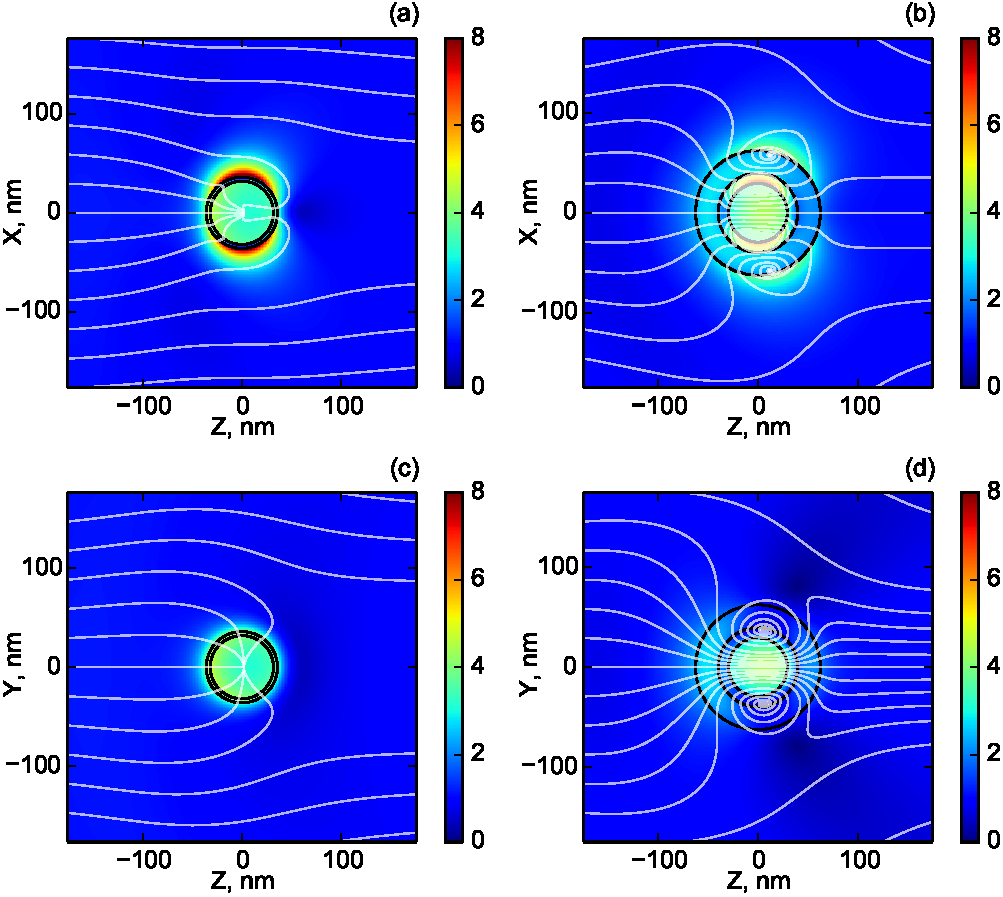
\includegraphics[width=0.47\textwidth]{fig/SiAgSi-flow-R62-YZ-Eabs.pdf}%
    \caption{ (Main field figure. The following figures are given for
      reference and should be removed from the manuscript). Electric
      field for efficient (a,c) and ``super'' (b,d) designs in E-k
      (a-b) and H-k (c-d) planes.
      \label{fig:Eabs}
    }%
  }
\end{figure}

\begin{figure}
  \center{
    % Use pdfcrop to remove white margins
    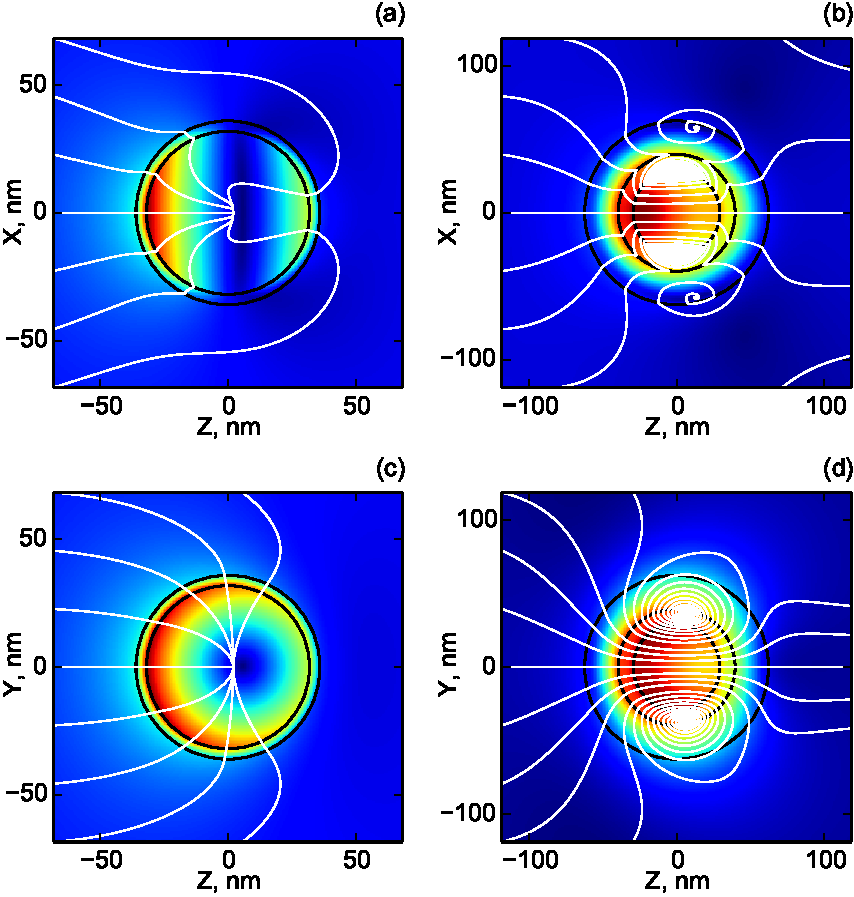
\includegraphics[width=0.47\textwidth]{fig/SiAgSi-flow-R62-YZ-Habs.pdf}%
    \caption{
      Same as Fig.~\ref{fig:Eabs} for magnetic field.
      %\label{fig:model-view}
    }%
  }
\end{figure}

\begin{figure}
  \center{
    % Use pdfcrop to remove white margins
    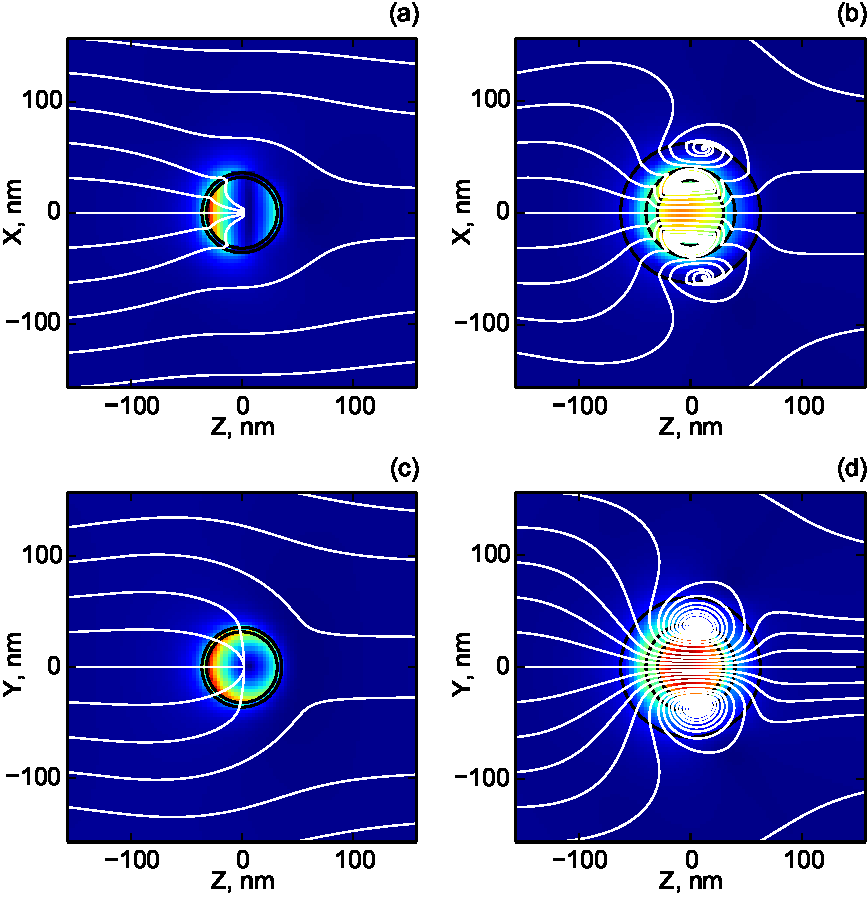
\includegraphics[width=0.47\textwidth]{fig/SiAgSi-flow-R62-YZ-Pabs.pdf}%
    \caption{ Same as Fig.~\ref{fig:Eabs} for Poynting vector.
      %\label{fig:model-view}
    }%
  }
\end{figure}

\begin{figure}
  \center{
    % Use pdfcrop to remove white margins
    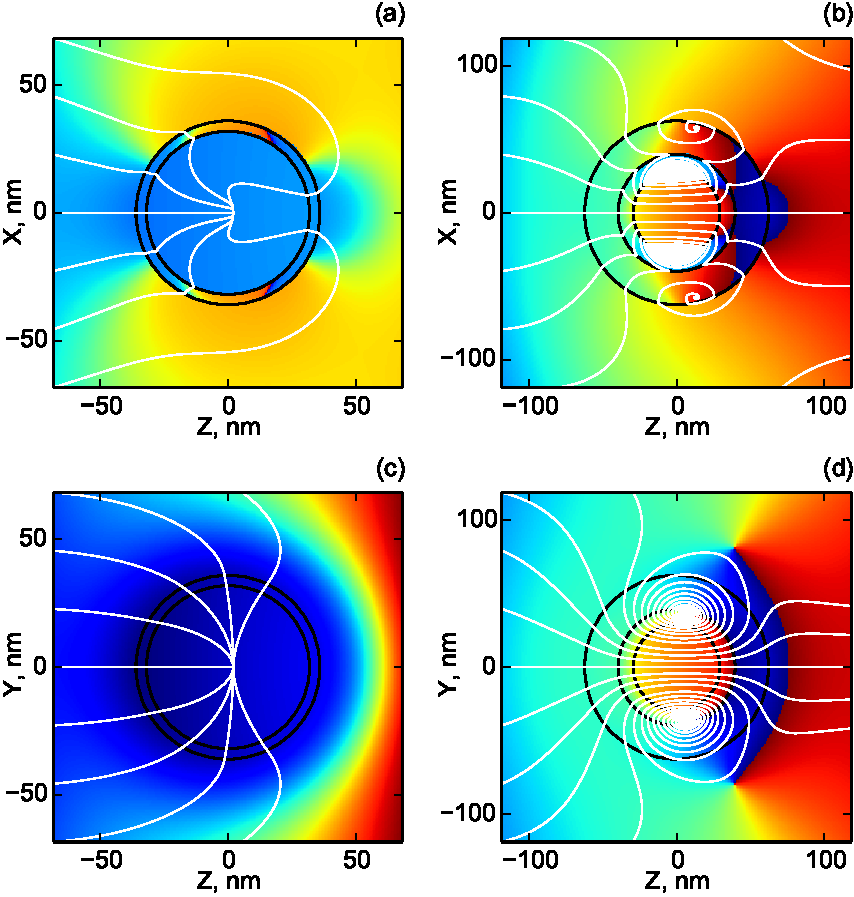
\includegraphics[width=0.47\textwidth]{fig/SiAgSi-flow-R62-YZ-angleEx.pdf}%
    \caption{ Same as Fig.~\ref{fig:Eabs} for phase of the electric
      field (x component).
      %\label{fig:model-view}
    }%
  }
\end{figure}

\begin{figure}
  \center{
    % Use pdfcrop to remove white margins
    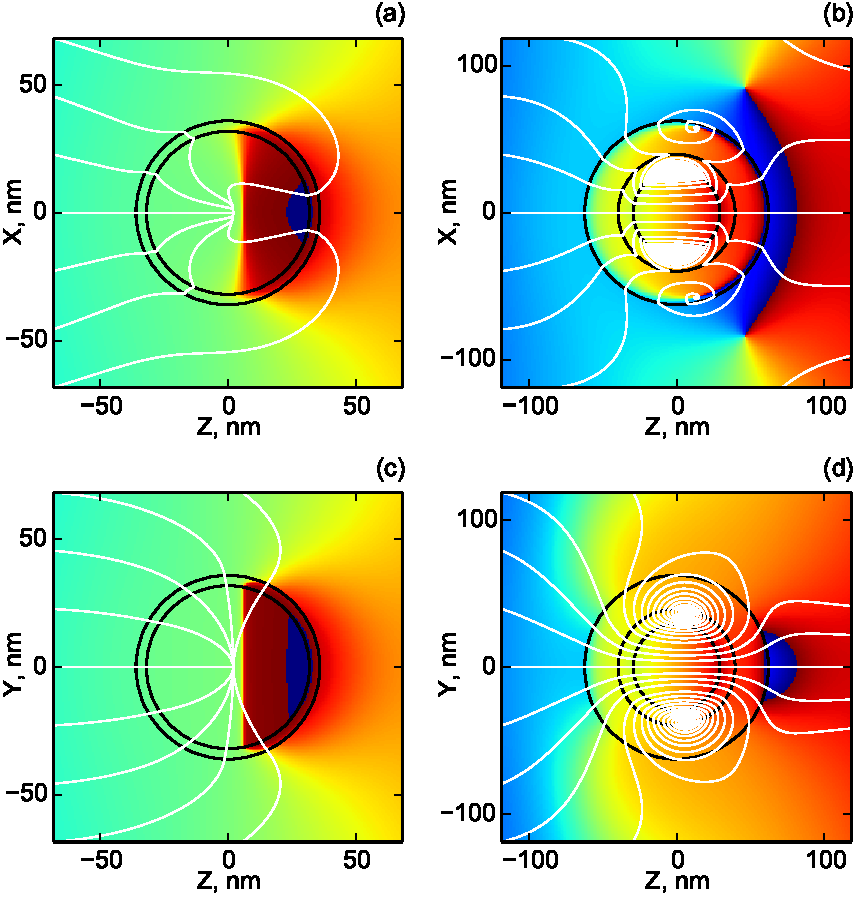
\includegraphics[width=0.47\textwidth]{fig/SiAgSi-flow-R62-YZ-angleHy.pdf}%
    \caption{ Same as Fig.~\ref{fig:Eabs} for phase of the magnetic
      field (y component).
      %\label{fig:model-view}
    }%
  }
\end{figure}




% In this work we propose to use isotropic nonmagnetic dielectric
% materials to design a multilayer spherical cloak embedded in a
% transparent medium (Fig.~\ref{fig:model-view}). As a first step,
% we set the optimizer to minimize radar cross section (RCS) from
% the cloaked target by changing layer normalized index values in
% the range from~0.67 to~8.  It is possible to implement in
% experiment the normalized index to have a value lower than unity
% by positioning low index material into the high index medium (solid or
% liquid).  The optimization index range used in our work is equivalent
% to layers index from~1 to~12 for the target hosted in the medium with
% index value of 1.5. Later on we use fixed index values of the layers
% and optimize layers width to minimize RCS.

% %\section{Methods}
% Mie theory based RCS calculations were evaluated with
% Scattnlay.~\cite{pena_scattering_2009} We used in-house
% developed~\cite{JADE-web} implementation of JADE+
% algorithm~\cite{Jingqiao-JADE-2009} for stochastic optimization with
% adaptive differential evolution approach. Final designs were verified
% by full-wave simulation in CST Microwave Studio\cite{CST-web}, total
% RCS value coincides with Mie calculation, relative difference is lower
% than 1\%.  Further details on the methodology used can be found
% elsewhere.~\cite{Ladutenko-2014}



% % \section{Optimization details}

% All simulations have been made for a target PEC (perfect electric
% conductor) sphere with $R = 0.75\lambda$, where $\lambda$ denotes the
% working wavelength.  RCS reference level obtained from bare target was
% 3.75~$\lambda^2$.
% % % Converting Radar Cross Section in Square Meters to Decibels dBsm =
% % % 10 x log10(RCS/1m2) dBsm: Radar Cross Section of target in decibels.
% % % RCS: Radar Cross Section of target in square meters.  EXAMPLE: What
% % % is the dBsm of a stealth fighter with a RCS of 0.01 m2?  10 x
% % % log10(0.01/1m2) = -20 dBsm
% Sphere was covered with a multilayer coating; for the first series of
% simulations, we divided the shell
% into 4, 8, and 16 layers of equal width.  Normalized refraction
% index for each layer was set independently. Total coating width
% was set in the range from zero to $W=0.24\lambda$.  Negligible loss
% was used in coating layers to increase numerical stability.  As a
% result we obtained many optimized designs (see
% Fig.~\ref{fig:rcs-overview-index07})
% \begin{figure}
%   \center{
%     \includegraphics[width=0.47\textwidth]{rcs-overview-index07}%
%     \caption{Final RCS after $\sim$1~400 optimization runs, bare
%       target RCS level is marked with a dot-dashed line.  Filled area
%       corresponds to threshold coating width for the single valley design
%       (like in Fig.~\ref{fig:index07-design}a and \ref{fig:index07-design}c)
%       studied in Ref~\onlinecite{Ladutenko-2014}.  Letters denote
%       designs selected for Fig.~\ref{fig:index07-design}.
%       \label{fig:rcs-overview-index07}}%
%     }
% \end{figure}
% for different coating width and number of layers in the coating.
% Optimization was repeated 12 times for each set of parameters;
% plotted marks represent the final result of a single run. Results
% can vary due to stochastic nature of the optimizer.
% %  Typical RCS reduction is about -60\%.
% %TODO дизайн *174955* - в начальном участоке всегда появляются слои
% %меньше 1, в целом в какой-то момент левый край становился меньше 1, а
% %для больших значений толщины покрытия у нас заваливается внешний край
% %и становится меньше 1.

%  \begin{figure}
%   \begin{minipage}[h]{0.235\textwidth}    \begin{flushleft}     a)    \end{flushleft}
%   \end{minipage}
%   \begin{minipage}[h]{0.235\textwidth}    \begin{flushleft}     b)    \end{flushleft}
%   \end{minipage}
%   \begin{minipage}[h]{0.235\textwidth} 
%    \includegraphics[width=0.95\textwidth]{index07-SV-best}
%   \end{minipage}
%   \begin{minipage}[h]{0.235\textwidth} 
%    \includegraphics[width=0.95\textwidth]{index07-DV}
%   \end{minipage}
%   \begin{minipage}[h]{0.235\textwidth}    \begin{flushleft}     c)    \end{flushleft}
%   \end{minipage}
%   \begin{minipage}[h]{0.235\textwidth}    \begin{flushleft}     d)    \end{flushleft}
%   \end{minipage}
%   \begin{minipage}[h]{0.235\textwidth} 
%    \includegraphics[width=0.95\textwidth]{index07-SV}
%   \end{minipage}
%   \begin{minipage}[h]{0.235\textwidth} 
%    \includegraphics[width=0.95\textwidth]{index07-TO}
%   \end{minipage}

%   \caption{Typical normalized 
% refractive index profiles selected from
% Fig.~\ref{fig:rcs-overview-index07}. 
% \label{fig:index07-design}}%
  
% \end{figure}
% We have identified a few typical patterns of design presented in
% Fig.~\ref{fig:index07-design}; all plots represent a design with a target
% PEC sphere to the left and the host medium to the right. Plotted index value is
% normalized to the host media index.  Designs in Fig.~\ref{fig:index07-design}(a-c)
% can be identified~\cite{Ladutenko-2014} as a single-valley and double-valley
% ones. Valley is a feature of index profile with a low index region bounded
% with high index. Visually valleys are easier to distinguish for designs with many
% layers (Fig.~\ref{fig:index07-design}b).  However, for a smaller number of layers
% the valley designs still exist and can be additionally identified in
% full-wave simulations and by spectral response.~\cite{Ladutenko-2014}
% Design in Fig.~\ref{fig:index07-design}a has the best performance (with -72.8\%
% of RCS drop).  Design in Fig.~\ref{fig:index07-design}c was verified
% with the full-wave simulation\cite{CST-web}, it has the similar phase
% switch inside the coating (see lower part of
% Fig.~\ref{fig:CST-E-field}a), which was discussed in details in
% Ref.~\onlinecite{Ladutenko-2014} using the scattering
% cancellation~\cite{alu} approach: we substitute negative electric
% susceptibility from quasistatic approximation with phase shift of wave
% inside the coating.  It leads to antiparallel direction of electric
% field in the inner and outer part of the coating, resulting in a
% reduced perturbation of the far field.  In contrast to Alu
% work~\cite{alu} with typical target $R$ less than 0.2~$\lambda$, we
% use several times larger target with $R=0.75\lambda$.

% Design in Fig.~\ref{fig:index07-design}d looks and performs differently.
% Wave inside and outside the coating travels in a joint manner
% (Fig.~\ref{fig:CST-E-field}b)
% \begin{figure}
%   \begin{minipage}[h]{0.47\textwidth}    \begin{flushleft}     a)    \end{flushleft}
%   \end{minipage}\\
%   \vspace{0.5em}
%   \begin{minipage}[h]{0.47\textwidth}
%   \center{
%     \includegraphics[width=1.0\textwidth]{CST-E-field-SV}%
%   }
%   \end{minipage}\\
%   \vspace{0.5em}
%   \begin{minipage}[h]{0.47\textwidth}    \begin{flushleft}     b)    \end{flushleft}
%   \end{minipage}\\
%   \vspace{0.5em}
%   \begin{minipage}[h]{0.47\textwidth}
%   \center{
%   \includegraphics[width=1.0\textwidth]{CST-E-field-DI}%
%   }
%   \end{minipage}
%     \caption{Distribution of electric field phase and
%     amplitude in H-k plane from CST simulation for (a) single valley
%     Fig.~\ref{fig:index07-design}c and (b) double index
%     Fig.~\ref{fig:index07-design}d design. Plane wave source
%     is to the left, borders of the outer
%     layer are marked with black circles. Phase is the lower part of the
%     image, degrees scale to the left, amplitude is the upper part,
%     scale to the right. 
%     \label{fig:CST-E-field}}%
% \end{figure}
% with some phase discontinuity on the boundaries of the high index layer.
% Such operation is similar to TO approach~\cite{pendry_TO}, however,
% the main TO feature is absent here.  In TO approach hidden object has
% the same phase all over the surface.  For the presented designs phase
% changes for almost two cycles on the surface during the passage of the
% wave.

% Presence of a new design type in Fig~\ref{fig:index07-design}d with use of
% normalized material index $<$1 causes four-layer design to be a
% preferable option to achieve minimal RCS for the total coating width
% less than $0.17\lambda$.  It is opposite to the results from
% Ref.~\onlinecite{Ladutenko-2014}, where it has been shown that four-layer
% designs of conventional dielectric material are not enough to
% form a distinguished single valley design, therefore, such designs do
% not reach common level of RCS reduction.  %TODO Alexander do not like
%                                 %world "common" in last sentence, any
%                                 %better word?

% Based on the design in Fig~\ref{fig:index07-design}d we have proposed double
% index~(DI) designs, where only two normalized index values $min$=0.67
% and $max$=8 are used; coating width of each layer was optimized to
% reduce RCS (with regard of constrain for the total coating width).  We have
% tested three design patterns of layers order in the coating:
% PEC-$max$-$min$, PEC-$min$-$max$, and PEC-$min$-$max$-$min$, target
% PEC is included into notation.  See
% Fig.~\ref{fig:rcs-overview-index07-DI} for final results of
% optimization and Fig.~\ref{fig:design-DI} for corresponding index
% designs of a triple layer structure (width of any layer was allowed to
% be zero).  We included value of RCS of a single layer coating with only
% $min$ index for reference.  It should be noted that such kind of
% design is preferred from the applied point of view, because it is
% much easier to control layer width than a material index.

% \begin{figure}
%   \center{
%     \includegraphics[width=0.47\textwidth]{rcs-overview-index07-DI}%
%       \caption{Double index designs trends overlaid on
%         Fig.~\ref{fig:rcs-overview-index07}, with previous data grayed
%         out.  
%         \label{fig:rcs-overview-index07-DI}}%
%     }
%   \center{
%     \includegraphics[width=0.47\textwidth]{design-DI}%
%       \caption{Double index designs for PEC-$min$-$max$-$min$, share of
%         total coating width for each layer is displayed. Transaction
%         from single to triple layer is shown in the inset.
%         \label{fig:design-DI}}%
% %todo triple layer добавить во вставку, цифры 1,0.
%  }
% \end{figure}

% There is a number of common features of DI designs, that can be noted
% in Fig.~\ref{fig:rcs-overview-index07-DI}.  For a very small total
% coating width (less than $0.03\lambda$) all DI patterns were optimized
% to the same design: there is a single layer of $min$ index, for all other
% layers the optimization process yielded a zero width. To make it clearer, the
% transaction of PEC-$min$-$max$-$min$ pattern from a single to triple
% layer is shown in the inset of Fig.~\ref{fig:design-DI}.  Double
% layer designs are also present in the inset for a very limited range
% of total coating width, where the outer $min$ layer width was
% optimized to be zero.

% It is interesting to mention that PEC-$max$-$min$ and
% PEC-$min$-$max$-$min$ patterns have a similar design for the total
% coating width larger than 0.2$\lambda$. The only notable difference
% between both designs is the presence of $min$ layer in contact with the
% target in triple layer structure, that shares less than 2\% of the
% total coating width.  The $max$ layer share is about 12\% for both
% patterns, the outer $min$ layers have similar share too.  However,
% presence of thin inner $min$ layer in triple layer pattern leads to a
% factor of two difference of RCS value for these two patterns. We have
% also tested 4-layer (PEC-$min$-$max$-$min$-$max$) and 5-layer
% (PEC-$min$-$max$-$min$-$max$-$min$) patterns with a hope to describe
% single valley designs. However, these additional DI patterns perform
% similar to triple layer DI pattern.



% % To study the origin of RCS reduction with high index layer we
% % calculated RCS patterns (Fig.~\ref{fig:rcs-pattern}) for optimized and
% % modified designs.
% \begin{figure}
%   \includegraphics[width=0.47\textwidth]{index07-spectra}%
%   \caption{RCS spectra for double index (DI) type and single valley
%     (SV) designs optimized at 1.0$\lambda$ wavelength.  Dashed line
%     spectrum is for the total RCS of a bare target. % lambda?
%     \label{fig:index07-spectra}}%
% \end{figure}
% \begin{figure}
%   % \begin{minipage}[h]{0.47\textwidth}    \begin{flushleft}     a)    \end{flushleft}
%   % \end{minipage}
%   % \begin{minipage}[h]{0.47\textwidth}
%     \center \includegraphics[width=0.45\textwidth]{RCS-bare-H-k-cloak-H-k}%
%   % \end{minipage}
%   % \begin{minipage}[h]{0.47\textwidth}    \begin{flushleft}      b)    \end{flushleft}
%   % \end{minipage}
%   % \begin{minipage}[h]{0.47\textwidth}
%   %   \includegraphics[width=0.7\textwidth]{RCS-bare-E-k-mod-cloak-E-k-mod}%
%   % \end{minipage}
%   \caption{Comparison of RCS pattern for a bare and cloaked target in
%     H-k plane of an optimized design from
%     Fig.~\ref{fig:index07-design}d. 
%     \label{fig:rcs-pattern}}%
% \end{figure}
% % Introduction of the high index second layer leads to significant
% % reduction of forward and backward scattering lobes with small increase
% % of side lobes.  Such a behavior reflects the fact, that second layer
% % can be treated as an impedance matcher.  It increases the share of
% % incident radiation, that penetrates into the coating, and, even more
% % important, induces high output of radiation from the coating in
% % forward direction.


% We should also notice a wide band performance of DI type cloaks, see
% Fig.~\ref{fig:index07-spectra} for cross section spectra.  Due to the
% use of dielectric materials for cloak layers and for the medium we do
% not take into account any dispersion.  Pendry TO
% cloak~\cite{pendry_TO} design does not depend on the wavelength of
% incident light.  Our DI type cloak (Fig.~\ref{fig:index07-design}d)
% has a band, however, it is about an order of magnitude larger than the
% band of single-valley design (Fig.~\ref{fig:index07-design}c).  For
% the selected cutting plane the RCS pattern in
% Fig.~\ref{fig:rcs-pattern} of the DI type cloak
% (Fig.~\ref{fig:index07-design}d) has a significant scattering
% reduction in all directions, especially in the forward one.

% %   Wide
% % band performance of proposed cloak can be related
% % with %TODO any other ideas?
% % 1) curvature of the impedance matching layer and the cloak itself, it
% % leads to a range of effective cloak thickness in the direction of the
% % incident radiation 2) close to the wavelength linear dimensions of the
% % cloak, which let to consider radiation interaction with the coating in
% % near-field regime.

% %\section{Conclusion}

% In summary, by using stochastic optimization we have designed
% multilayer shells composed of isotropic nonmagnetic dielectric
% materials; these shells provide scattering reduction on targets
% embedded in a transparent medium.  Two types of designs have been
% identified; the first one has a wide band performance and can be
% approximated with a double index design, whereas the other can be
% described in terms of scattering cancellation theory and consists in
% single and double valley designs. For a target with diameter
% of~1.5~$\lambda$ scattering has been reduced with these cloak types
% by~57\% and~72\%, respectively. We analyzed several double index
% patterns; optimized designs with PEC-$min$-$max$-$min$ pattern
% were found to produce better scattering reduction performance than
% designs with fixed layer width when total coating width is small.

% Fundamental Limits to Extinction by Metallic Nanoparticles
% Phys. Rev. Lett. 112, 123903 – Published 26 March 2014 O. D. Miller,
% C. W. Hsu, M. T. H. Reid, W. Qiu, B. G. DeLacy, J. D. Joannopoulos,
% M. Soljačić, and S. G. Johnson

% \begin{acknowledgments}
%   The authors would like to thank the Ministry of Education and
%   Science of the Russian Federation (Goszadanie 2014/190, Zadanie
%   No. 3.561.2014/K, project 14.584.21.0009 10), Russian Foundation for Basic
%   Research (Grant 15-02-01344), and Government of the Russian
%   Federation (Grant 074-U01) for the financial support. The
%   simulations of cloak designs has been funded by the Russian Science
%   Foundation Grant No. 14-12-01227.% We
%   % would also like to appreciate Alexander Krasnok for the help with
%   % CST simulations and Ilya V. Shadrivov for valuable comments on the
%   % manuscript.
% \end{acknowledgments}

\bibliography{2015-Ladutenko-Qabs}
\end{document}

